\documentclass[a4paper]{article}
\usepackage{graphicx}
\usepackage{float}
\usepackage{pgfplots}
\pgfplotsset{compat=1.18}
\usepackage{listings}
\usepackage{enumitem}
\usepackage{cancel}
\usepackage{amsmath}
\usepackage{amsthm}
\usepackage{amssymb}
\usepackage{pgfplots}
\usepackage{mdframed}
\usepackage{lipsum}
\newmdtheoremenv{theo}{Theorem}
\usepackage{mdframed} 

% Define theorem styles
\newtheorem{theorem}{Theorem}[section]    % Theorems numbered within sections
\newtheorem{lemma}[theorem]{Lemma}        % Lemmas use the same counter as theorems
\newtheorem{corollary}[theorem]{Corollary} % Corollaries use the same counter as theorems
\newtheorem{proposition}[theorem]{Proposition} % Proposition uses the same counter
\newtheorem{property}[theorem]{Propriety}
\theoremstyle{definition}
\newtheorem{definition}[theorem]{Definition}

% Remark-style theorem
\theoremstyle{remark}
\newtheorem{remark}[theorem]{Remark}

% Boxed environment for theorems
\newmdenv[
  linewidth=0.8pt,
  roundcorner=5pt,
  linecolor=black,
  backgroundcolor=white!5,
  skipabove=\baselineskip,
  skipbelow=\baselineskip,
  innerleftmargin=10pt,
  innerrightmargin=10pt,
  innertopmargin=5pt,
  innerbottommargin=5pt
]{thmbox}

% Custom proof environment (also boxed)
\renewenvironment{proof}[1][Proof]{%
  \begin{mdframed}[linewidth=0.8pt, roundcorner=5pt, linecolor=black, skipabove=\baselineskip, skipbelow=\baselineskip, innertopmargin=5pt, innerbottommargin=5pt]%
  \noindent\textbf{#1. }%
}{%
  \end{mdframed}%
}

% Redefine theorem environments to use thmbox
\let\oldtheorem\theorem
\renewenvironment{theorem}{\begin{thmbox}\begin{oldtheorem}}{\end{oldtheorem}\end{thmbox}}

\let\oldlemma\lemma
\renewenvironment{lemma}{\begin{thmbox}\begin{oldlemma}}{\end{oldlemma}\end{thmbox}}

\let\oldcorollary\corollary
\renewenvironment{corollary}{\begin{thmbox}\begin{oldcorollary}}{\end{oldcorollary}\end{thmbox}}

\let\oldproposition\proposition
\renewenvironment{proposition}{\begin{thmbox}\begin{oldproposition}}{\end{oldproposition}\end{thmbox}}

\let\oldproperty\property
  \renewenvironment{property}{\begin{oldproperty}}{\end{oldproperty}}


% Reference shortcuts
\newcommand{\thmref}[1]{Theorem~\ref{#1}}
\newcommand{\lemref}[1]{Lemma~\ref{#1}}
\newcommand{\corref}[1]{Corollary~\ref{#1}}
\newcommand{\propref}[1]{Property~\ref{#1}} 

% To customize QED symbol
\renewcommand{\qedsymbol}{$\blacksquare$}


\usepackage{tikz-cd}

\usetikzlibrary{decorations.pathreplacing} % for angle arc
\usetikzlibrary{angles, quotes, calc} % for drawing angles

\usepackage{color}   %May be necessary if you want to color links
\usepackage{hyperref}
\hypersetup{
    colorlinks=true, %set true if you want colored links
    linktoc=all,     %set to all if you want both sections and subsections linked
    linkcolor=black,  %choose some color if you want links to stand out
}

\usepackage{xcolor}
\usepackage{tcolorbox}
% Define a custom tcolorbox environment for examples
\newtcolorbox{examplebox}[2][]{
  colback=blue!5!white,   % Background color
  colframe=blue!30!black, % Border color
  title=#2,          % Title of the box
  boxrule=0mm,          % Thickness of the border                % Rounded corners
  fonttitle=\bfseries,    % Title font style
  width=\textwidth,  
  #1 % Width of the box (adjustable)
}

\definecolor{codegreen}{rgb}{0,0.6,0}
\definecolor{codegray}{rgb}{0.5,0.5,0.5}
\definecolor{codepurple}{rgb}{0.58,0,0.82}
\definecolor{backcolour}{rgb}{0.95,0.95,0.92}

\lstdefinestyle{mystyle}{
    backgroundcolor=\color{backcolour},   
    commentstyle=\color{codegreen},
    keywordstyle=\color{magenta},
    numberstyle=\tiny\color{codegray},
    stringstyle=\color{codepurple},
    basicstyle=\ttfamily\footnotesize,
    breakatwhitespace=false,         
    breaklines=true,                 
    captionpos=b,                    
    keepspaces=true,                 
    numbers=left,                    
    numbersep=5pt,                  
    showspaces=false,                
    showstringspaces=false,
    showtabs=false,                  
    tabsize=2
}

\lstset{style=mystyle}

\makeatletter
\renewcommand*\env@matrix[1][*\c@MaxMatrixCols c]{%
  \hskip -\arraycolsep
  \let\@ifnextchar\new@ifnextchar
  \array{#1}}
\makeatother
\usepackage{tikz}
\usepackage{booktabs}
\title{Sistemi}
\author{Università di Verona\\Imbriani Paolo -VR500437\\Professor Francesco Visentin}

\begin{document}

\begin{figure}
    \centering
    \includegraphics[width=0.3\textwidth]{UniversityofVerona.png}
    \label{fig:centered-image}
\end{figure}

\maketitle 

\pagebreak

\tableofcontents

\pagebreak

\section{Trasformata di Laplace}

\begin{definition}
$v(t)$ è definito nel tempo. V(s) è la sua trasformata. 
    \[\mathcal{L}[f(t)](s) = \int_{0}^{+\infty} v(t)e^{-st}dt\]
\end{definition}

\begin{figure}[H]
    \centering
    \caption{$\alpha \ge max\{\lambda_i\}$}
    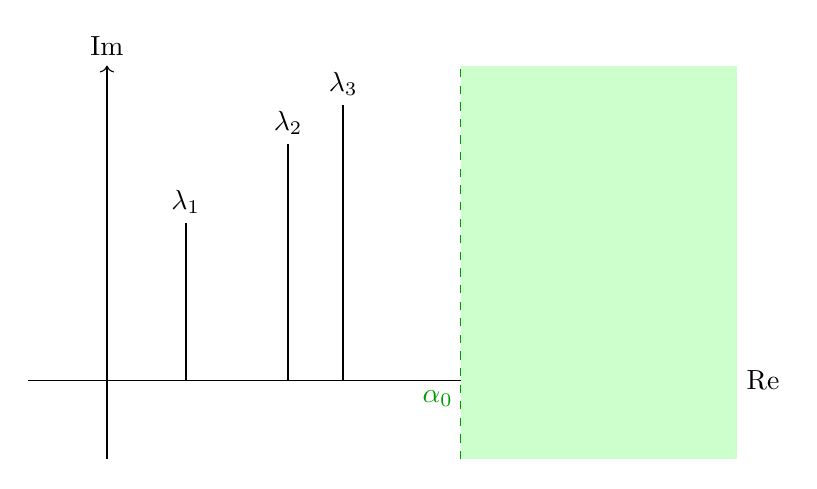
\begin{tikzpicture}
        % Axes
        \draw[->] (-1, 0) -- (8, 0) node[right] {$\operatorname{Re}$};
        \draw[->] (0, -1) -- (0, 4) node[above] {$\operatorname{Im}$};
    

        \draw[thick] (1, 0) -- (1, 2);
        \node[above] at (1, 2) {$\lambda_1$};
        \draw[thick] (2.3, 0) -- (2.3, 3);
        \node[above] at (2.3, 3) {$\lambda_2$};
        \draw[thick] (3, 0) -- (3, 3.5);
        \node[above] at (3, 3.5) {$\lambda_3$};
    
        % Dashed line for region boundary at x = 4.5
        \draw[dashed, thick, green!60!black] (4.5, -1) -- (4.5, 4);
        \node[below, green!60!black] at (4.2, 0) {$\alpha_0$};
    
        % Green filled region of convergence
        \fill[green!20] (4.5, -1) rectangle (8, 4);

    \end{tikzpicture}
\end{figure}


\subsection{Proprietà}

La trasformata di LaPlace ha svariate utili proprietà che possiamo utilizzare a nostro vantaggio:
\indent
\begin{property}
\label{prop:linearity_lap}
    \textbf{Linearità}: \[a_1v_1(t) + a_2v_2(t) = a_1V_1(s) + a_2V_2(s)\]
\end{property}
\begin{property}
\label{prop:traslas_time_lap}
    \textbf{Traslazione nel dom. del tempo: } \[\mathcal{L}[v(t-\tau)](s) = \overbrace{e^{-st}V(s)}^{\tau > 0}\]
\end{property}
\begin{property}
\label{prop:traslas_compl_lap}
    \textbf{Tralaslazione nel dom. dei complessi: }
    \[\mathcal{L}[e^{\lambda t}v(t)] = V(s - \lambda)\]
\end{property}
\begin{property}
\label{prop:cambio_di_scala}
    \textbf{Cambio di scala:}
    \[\mathcal{L}[v(rt)](s) = \frac{1}{r}V\left(\frac{s}{r}\right)\]
\end{property}
\begin{property}
\label{prop:derivata_lap}
    \textbf{Proprietà delle derivate:} Se $v(t)$ ammette TdL (Trasformata di Laplace) ed esiste finito $v(0^-) = \lim_{t \rightarrow 0} v(t)$ 
    allora anche la sua derivata i-esima ammette TdL.
    \[\mathcal{L}\left[\frac{d^iv(t)}{dt}\right] = S^iV(s) - \sum_{k = 0}^{i-1} \frac{d^kv(t)}{d^t}\bigg|_{t = 0^-} (S^{i-1-k})\]
\end{property}
\begin{proof}
    Per la derivata prima:
    \begin{align*}
        \mathcal{L}\left[\frac{d}{dt}v(t)\right](s) &= \int_{0}^{\infty} \frac{d}{dt}v(t)e^{-st}dt =\\ 
        &= v(t)e^{-st}\bigg|_0^{+\infty} + s\int_{0}^{\infty}v(t)e^{-st}dt\\
        &= \lim_{\varepsilon \rightarrow 0} v(\varepsilon)e^{-s\varepsilon} - \lim_{\varepsilon \rightarrow 0^-} v(\varepsilon)e^{-s\varepsilon} + sV(s)\\
        &= sV(s) - v(0^-)
    \end{align*}
\end{proof}
\begin{proof}
    Per la derivata seconda:
    \begin{align*}
        \mathcal{L}\left[\frac{d^2}{dt^2}v(t)\right](s) &= \mathcal{L}\left[\frac{d}{dt}\left(\frac{d}{dt}v(t)\right)\right](s)\\  &= s\mathcal{L}\left[\frac{d}{dt}v(t)\right](s) - \frac{d}{dt} v(t)\bigg|_{t = 0^-}\\
        &= \int_{0}^{+\infty} \left[S\mathcal{L}[v(t)](s) - v(0^-)\right] - \frac{d}{dt}v(t)\bigg|_{t = 0^-}\\
        &= s^2V(s) - sv(0^-) - \frac{d}{dt}v(t)\bigg|_{t = 0^-}
    \end{align*}
\end{proof}
\begin{property}
    \label{prop:molt_funz_pol}
    \textbf{Moltiplicazione per funzioni polinomiali:} Se $v(t)$ ammette TdL e t è un polinomio allora anche $tV(s)$ ammette TdL.
    \[\mathcal{L}[t^iv(t)](s) = (-1)^i\frac{d^iV(s)}{dS^i}\]
\end{property}
\begin{proof}
    \textbf{Per $i = 1$}: 
    \begin{align*}
        \mathcal{L}[tv(t)](s) = \int_{0^-}^{+\infty} tv(t)e^{-st}dt &= -\int_{0^-}^{+\infty}v(t) \cdot (te^{-st})dt\\
        &= -\int_{0}^{+\infty} v(t)\frac{d}{ds}te^{-st}dt \\
        &= -\frac{d}{ds}\overbrace{\int_{0}^{\infty}v(t)e^{-st}dt}^{\text{TdL}}\\
        &= -\frac{d}{ds}V(s)
    \end{align*}
\end{proof}
\begin{property}
    \textbf{Integrazione nel dom. del tempo}: Se $v(t)$ ammette TdL, allora $\Psi(t) = \int_{0^-}^{t}v(t)dt$ ammette TdL
    \[\mathcal{L}[\Psi(t)](s) = \frac{V(s)}{s}\]
    Ascissa di convergenza: $\alpha = max\{0, \alpha_0\}$
\end{property}
\begin{proof}
    \begin{align*}
        v_1(t) = \int_{0^-}^{\infty} v(t)dt \Longrightarrow \begin{cases}
            v_1' = v(t)\\
            v(0^-) = \int_{0^-}^{0^-}v(t)dt = 0
        \end{cases}
    \end{align*}
    \begin{align*}
        V(s) = \mathcal{L}[v(t)](s) &= \mathcal{L}[v_1'(t)](s) = S\mathcal{L}[v_1'(t)](s) - v_1(0^-)\\
        &= \mathcal{L}\left[\int_{0}^{t}v(t)dt\right](s)\\ &= \frac{V(s)}{s}
    \end{align*}
\end{proof}
\begin{property}
    \textbf{Integrazione nel dom. dei complessi}: Se $v(t)$ ammette TdL e esiste $\lim_{t \rightarrow 0^-}\frac{v(t)}{t}$
    allora:
    \[\mathcal{L}\left[\frac{v(t)}{t}\right](s) = \int_{s}^{\infty} \mathcal{L}[v(t)](\zeta)d\zeta\]
\end{property}
\begin{proof}
    \begin{align*}
        \int_{s}^{+\infty} \mathcal{L}[v(t)](\zeta)d\zeta &= \int_{s}^{\infty} \int_{0^-}^{\infty} v(t)e^{-st} dtd\zeta\\
        &= \int_{0^-}^{\infty} v(t)\underbrace{\left(\int_{s}^{+\infty}e^{-t\zeta}d\zeta\right)}_{= \frac{e^{-st}}{t}}dt\\
        &= \int_{0}^{\infty}\frac{v(t)}{t}e^{-st}dt = \mathcal{L}\left[\frac{v(t)}{t}\right](s)
    \end{align*}
\end{proof}
\begin{theorem}
    \label{thm:val_iniziale_lap} \textbf{Teorema del valore iniziale}:
    Se $v(t)$ ammette TdL ed esiste finito $\lim_{t \rightarrow 0^-}v(t)$ allora 
    \[\lim_{t \rightarrow 0^-} v(t) = \lim_{s \rightarrow \infty} S\mathcal{L}[v(t)](s)\]
\end{theorem}
\begin{theorem}
    \label{thm:val_finale_lap} \textbf{Teorema del valore finale}:
    Se $v(t)$ ammette TdL ed esiste finito $\lim_{t \rightarrow \infty}v(t)$ allora 
    \[\lim_{t \rightarrow \infty} v(t) = \lim_{s \rightarrow 0^+} S\mathcal{L}[v(t)](s)\]
\end{theorem}
\begin{property}
    \textbf{Convoluzione nel dom. del tempo}: Siano $u(t)$ e $v(t)$ due funzioni causali (nulla per $t<0$) che ammettono TdL, allora la loro convoluzione $(u \ast v)(t)$ ammette TdL. 
    \[\mathcal{L}[(u \ast v)(t)](s) = \mathcal{L}[u(t)](s) \cdot \mathcal{L}[v(t)](s)\]
\end{property}
\begin{proof}
    \begin{align*}
        \mathcal{L}[(u \ast v)(t)](s) &= \int_{0}^{+\infty} (u \ast v)(t)e^{-st}dt\\
        &= \int_{0}^{+\infty} \left(\int_{0}^{t}u(\tau)v(t-\tau)d\tau\right)e^{-st}dt\\
        &= \int_{0}^{+\infty} \int_{0}^{t}u(\tau)v(t-\tau)e^{-st}d\tau dt\\
        &= \int_{0^-}^{\infty} u(\tau)\left(\int_{0^-}^{\infty} v(t-\tau)e^{-st}dt\right)d\tau\\
    \end{align*}
    Sostituiamo $x = t - \tau \rightarrow t = x + \tau \rightarrow dt = dx$ 
    \begin{align*}
        &= \int_{0^-}^{\infty} u(\tau)\left(\int_{0^-}^{\infty} v(x)e^{-s(x+\tau)}dx\right)d\tau\\ 
        &= \int_{0}^{+\infty} u(\tau)e^{-s\tau}d\tau \cdot \int_{0}^{+\infty}v(x)e^{-sx}dt\\
        &= \mathcal{L}[u(t)](s) \cdot \mathcal{L}[v(t)](s)
    \end{align*}
\end{proof}

\subsection{Trasformate di funzioni notevoli}
Ora andremo a vedere le trasformate di alcune funzioni notevoli:\\
Trasformata dell'\textbf{impulso unitario}:

\begin{figure}[H]
    \centering
\begin{tikzpicture}
    % Unitary Impulse Function (Delta Function)

        % Axes
        \draw[->] (-2, 0) -- (2, 0) node[right] {$t$};
        \draw[->] (0, -0.5) -- (0, 2) node[above] {$\delta(t)$};

        % Impulse at t = 0
        \draw[thick, ->] (0, 0) -- (0, 1.5);
        \node[above] at (0, 1.5) {$1$};

        % Labels
        \node[below left] at (0, 0) {$0$};
        \node at (0, -1) {Unit Impulse $\delta(t)$};
\end{tikzpicture}
\end{figure}

\[\mathcal{L}[\delta(t)](s) = \int_{0}^{+\infty} \delta(t)e^{-st}dt = e^{-s \cdot 0} = 1\]
Ampiezza:
\[\mathcal{L}[A\delta_0(t)](s) = A\overbrace{\cancel{\mathcal{L}[\delta_0(t)](s)}}^{1} = A\]
Ritardato nel tempo:
\[\mathcal{L}[\delta(t-\tau)](s) = e^{-st}\mathcal{L}[\delta_0(t)](s) = e^{-s\tau}\]

\begin{figure}[H]
    \centering
    \begin{tikzpicture}
    % Space between the graphs
        % Unit Step Function (Heaviside Function)
        % Axes
        \draw[->] (-2, 0) -- (2, 0) node[right] {$t$};
        \draw[->] (0, -0.5) -- (0, 2) node[above] {$u(t)$};

        % Step function
        \draw[thick] (-2, 0) -- (0, 0);
        \draw[thick] (0, 1) -- (2, 1);
        \draw[fill=white] (0, 1) circle (2pt);  % Open circle at t=0
        \node[left] at (0, 1) {$1$};

        % Labels
        \node[below left] at (0, 0) {$0$};
        \node at (0, -1) {Unit Step $u(t)$};
\end{tikzpicture}
\end{figure}

\begin{align*}
    \mathcal{L}[\delta_{-1}(t)](s) &= \int_{0^-}^{\infty} \delta_{-1}(t)e^{-st}dt\\
    &= \int_{0^-}^{\infty}e^{-st}dt \\
    &= \frac{e^{-st}}{-s}\bigg|_{0^-}^{\infty} = \frac{1}{s}
\end{align*}
\begin{align*}
    \mathcal{L}[A\delta_{-1}(t)](s) &= A\mathcal{L}[\delta_{-1}(t)](s) = \frac{A}{s}\\
    &= \mathcal{L}[\delta_{t - \tau}](s) \\
    &= e^{-s\tau}\mathcal{L}[\delta_{-1}(t)](s) \\
    &= \frac{e^{-s\tau}}{s}
\end{align*}
\noindent
\textbf{Esponenziale complesso causale}: $v(t) = e^{\lambda t}\delta_{-1}(t)$

\begin{figure}[H]
\centering
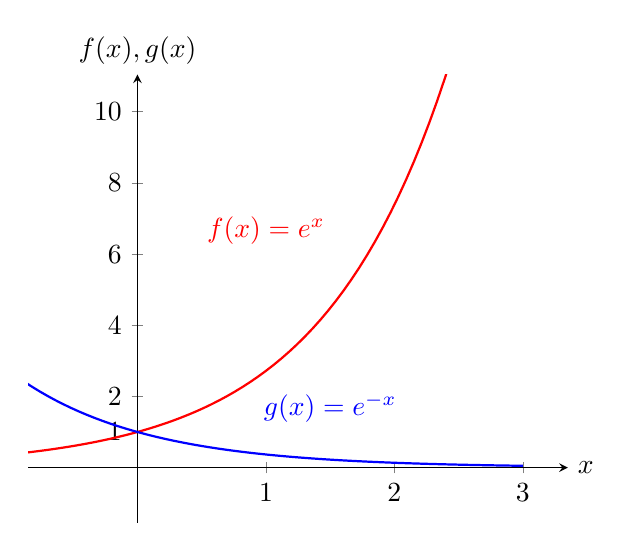
\begin{tikzpicture}
    \begin{axis}[
        axis lines = middle,
        xlabel = {$x$},
        ylabel = {$f(x), g(x)$},
        xmin = -0.5, xmax = 3,
        ymin = -0.5, ymax = 10,
        samples = 100,
        domain = -3:3,
        every axis x label/.style={at={(current axis.right of origin)}, anchor=west},
        every axis y label/.style={at={(current axis.above origin)}, anchor=south},
        xtick={-3,-2,-1,0,1,2,3},
        ytick={1,2,4,6,8,10},
        enlargelimits
    ]

        % Plot of e^x (exponential growth)
        \addplot[thick, red] {exp(x)};
        \node[red, above] at (axis cs:1,6) {$f(x) = e^x$};

        % Plot of e^-x (exponential decay)
        \addplot[thick, blue] {exp(-x)};
        \node[blue, above] at (axis cs:1.5,1) {$g(x) = e^{-x}$};

    \end{axis}
\end{tikzpicture}
\end{figure}


\begin{align*}
    \mathcal{L}[e^{\lambda t}\delta_{-1}(t)](s) &= \mathcal{L}[\delta_{-1}(t)](s - \lambda) \\
    &= \frac{1}{s - \lambda}
\end{align*}
\[\mathcal{L}[Ae^{\lambda t}\delta_{-1}(t)](s) = \frac{A}{s-\lambda}\]
\[\mathcal{L}[e^{\lambda(t - \tau)}\delta_{-1}(t - \tau)](s) = \frac{e^{-(s-\lambda)\tau}}{s-\lambda}\]
\textbf{Esponenziale complesso causale moltiplicato per una funzione polinomiale}: \[v(t) = \frac{t^l}{l!}e^{\lambda t}\delta_{-1}(t)\]


\begin{align*}
    \mathcal{L}\left[\frac{t^l}{l!}e^{\lambda t}\delta_{-1}(t)\right](s) &= \frac{1}{l!}\mathcal{L}[t^l e^{\lambda t}\delta_{-1}(t)](s)\\
    &\stackrel{\ref{prop:traslas_time_lap}}{=} \frac{(-1)^l}{l!}\frac{d^l}{dS^l}\mathcal{L}[e^{\lambda t}\delta_{-1}(t)](s)\\
    &= \frac{(-1)^l}{l!}\frac{d^l}{dS^l}\frac{1}{s-\lambda}\\
    &= \frac{(-1)^l}{l!}\frac{l! (-1)^l}{(s-\lambda)^{l+1}}\\
    &= \frac{1}{(s-\lambda)^{l+1}}
\end{align*}
\begin{examplebox}{Esempio 1}
    Con l = 1 
    \[\mathcal{L}[te^{e^{\lambda t}}\delta_{-1}(t)](s) = \frac{1}{(s-\lambda)^2}\]
    Con l = 2
    \[\mathcal{L}\left[\frac{t^2}{2!}e^{\lambda t}\delta_{-1}(t)\right](s) = \frac{1}{(s-\lambda)^3}\]
\end{examplebox}
\noindent
\textbf{Funzione coseno}:
\begin{figure}[H]
    \centering
    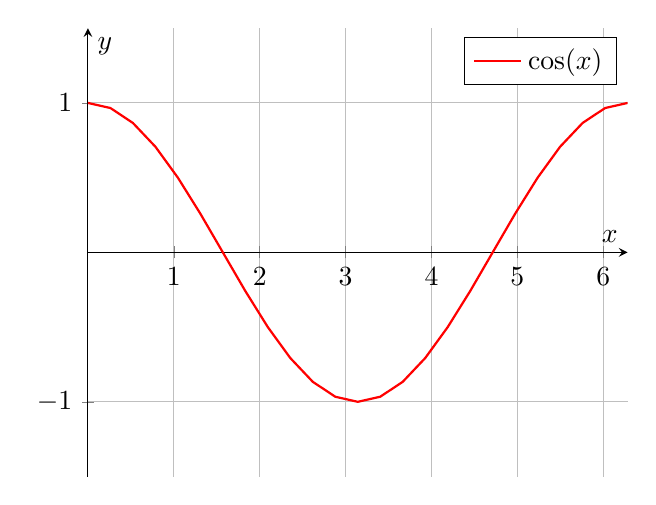
\begin{tikzpicture}
        \begin{axis}[
            axis lines = middle, 
            xlabel={$x$}, ylabel={$y$},
            domain=0:2*pi, 
            grid=both,
            xmin=0, xmax=2*pi, ymin=-1.5, ymax=1.5
        ]
            \addplot[red, thick] {cos(deg(x))};
            \legend{$\cos(x)$}
        \end{axis}
        \end{tikzpicture}
\end{figure}
\begin{align*}
\mathcal{L}[cos(wt)](s) &\stackrel{Eulero}{=} \mathcal{L}\left[\frac{e^{jwt} - e^{-jwt}}{2}\right]\\
&= \frac{1}{2}\left[\mathcal{L}[e^{jwt}](s) - \mathcal{L}[e^{-jwt}](s)\right] \\
&= \frac{1}{2}\left[\frac{1}{s-jw} + \frac{1}{s+jw}\right] \\
&= \frac{s}{s^2 + w^2}
\end{align*}
\textbf{Funzione seno}:
\begin{figure}[H]
    \centering
    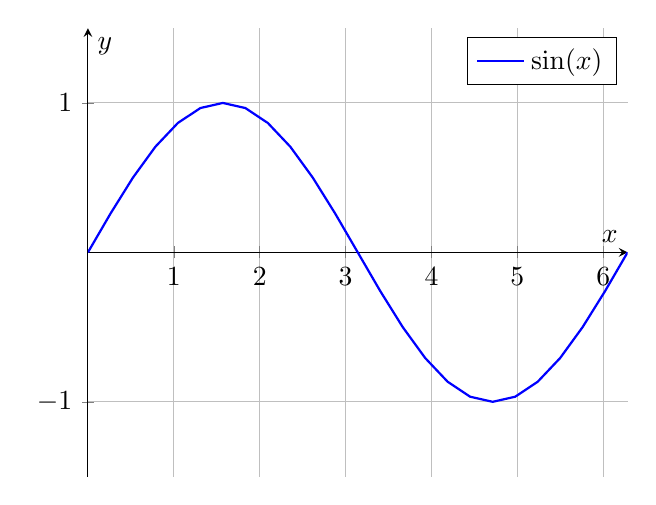
\begin{tikzpicture}
        \begin{axis}[
            axis lines = middle, 
            xlabel={$x$}, ylabel={$y$},
            domain=0:2*pi, 
            grid=both,
            xmin=0, xmax=2*pi, ymin=-1.5, ymax=1.5
        ]
            \addplot[blue, thick] {sin(deg(x))};
            \legend{$\sin(x)$}
        \end{axis}
        \end{tikzpicture}
\end{figure}
\begin{align*}
    \mathcal{L}[sin(wt)](s) &\stackrel{Eulero}{=} \mathcal{L}\left[\frac{e^{jwt} - e^{-jwt}}{2j}\right]\\
    &= \frac{1}{2j}\left[\mathcal{L}[e^{jwt}](s) - \mathcal{L}[e^{-jwt}](s)\right] \\
    &= \frac{1}{2j}\left[\frac{1}{s-jw} - \frac{1}{s+jw}\right] \\
    &= \frac{1}{2j}\left[\frac{\cancel{s}+jw - \cancel{s}+jw}{s^2 + w^2}\right] \\
    &= \frac{w}{s^2 + w^2}
\end{align*}

\subsection{Applicazione della TdL per i sistemi LTI causali}
\begin{equation*}
    \color{red}
    \sum_{i=0}^{n} a_i \frac{d^iv(t)}{dt^i} = \sum_{i=0}^{m} b_i \frac{d^iu(t)}{dt^i}
\end{equation*}
\[n \ge m \text{ e } u(t) = u(t)\cdot \delta_{-1}(t) (u(t)=0, t<0)\]
E consideriamo le n-1 condizioni iniziali:
\[v(0^-), \; \frac{dv(0)}{dt}; \; \frac{d^2v(0)}{dt^2}; \; \dots \; \frac{d^{n-1}v(0)}{dt^{n-1}}\]
Se $u(t)$ ammette TdL allora anche $v(t)$ ammette TdL e:
\begin{equation*}
    \mathcal{L}\left[\sum_{i=0}^{n} a_i \frac{d^iv(t)}{dt^i}\right](s) = \mathcal{L}\left[\sum_{i=0}^{m} b_i \frac{d^iu(t)}{dt^i}\right](s)
\end{equation*}
\begin{equation*}
    \sum_{i=0}^{n} a_i \mathcal{L}\left[\frac{d^iv(t)}{dt^i}\right](s) = \sum_{i=0}^{m} b_i \mathcal{L}\left[\frac{d^iu(t)}{dt^i}\right](s)
\end{equation*}
Applicando $n+m$ volte la regole della derivata:\\
\begin{align*}
   &a_n\left[S^nV(s) - \sum_{k=0}^{n-1}\frac{d^kv(t)}{dt^k}\bigg|_{t=0^-}(S^{n-1-k})\right] + \\
   &+ a_{n-1}\left[S^{n-1}V(s) - \sum_{k=0}^{n-2}\frac{d^kv(t)}{dt^k}\bigg|_{t=0^-}(S^{n-2-k})\right] +\\
   &+ \dots + a_0V(s)\\
   &= b_mS^mU(s) + b_{m-1}S^{m-1}U(s) + \dots + b_0U(s)
\end{align*}
Imponiamo le C.I.: $u(t)\bigg|_{t=0} = 0$\\\\
Espandiamo e raccogliamo:
\begin{align*}
    &\underbrace{\left[a_nS^n + a_{n-1}S^{n-1} + \dots + a_0\right]V(s)}_{d(s)} +\\
    &- \underbrace{a_nv(0^-)S^{n-1}\left(a_{n-1}v(0^-) + a_n\frac{dv(t)}{dt}\bigg|_{t=0^-}\right) - \; \dots \; - \left(\sum_{k=0}^{n-1} a_{k+1} \frac{d^kv(t)}{dt^k}\bigg|_{t=0^-}\right)}_{p(s)}\\
    &= \underbrace{(b_mS^m + b_{m-1}S^{m-1} + \dots + b_0)}_{n(s)}U(s)
\end{align*}

\[\Longrightarrow d(s) \cdot V(s) - p(s) = n(s) \cdot U(s)\]
\[V(s) = \frac{n(s)}{d(s)} \cdot U(s) + \frac{P(s)}{d(s)}\]
\begin{itemize}
    \item \textcolor{green!70!black}{$n(s)$} è un polinonio di grado $m$
    che dipende solo dai coefficenti delle derivate associate all'ingresso. \colorbox{blue!30!white}{Polinimonio caratteristico di u(t)}
    \item \textcolor{green!70!black}{$d(s)$} è un polinomio di grado $n$ che dipende
    solo dai coefficenti delle derivate associate di uscita. \colorbox{blue!30!white}{Polinimonio caratteristico di v(t)}
    \item \textcolor{green!70!black}{$p(s):$}\[\sum_{k=0}^{n-1}S^k\left(\sum_{j=k+1}^{n} a_{j+1} \frac{d^{n-j}}{dt^{n-j}}\bigg|_{t=0^-}\right)\]
    Polinomio di grado $n-1$ che dipende solo dalle C.I di v(t)
    \item \textcolor{green!70!black}{$\frac{P(s)}{d(S)}$} è una funzione razionale che dipende solo dalle C.I ì del sistema e dai 
    coefficenti del polinomio caratteristico di $v(t)$
    \[V_l(s) = \frac{P(s)}{d(s)}\]
    \item \textcolor{green!70!black}{$\frac{n(s)}{d(s)}U(s)$} è una funzione razionale che dipende dai coefficenti
    del polinomio caratteristico di $u(t)$, dei coefficenti del polinomio caratteristico di v(t) moltiplicati per tali u(t):
    \[V_f(s) = \frac{n(s)}{d(s)}U(s)\]
    \item \textcolor{green!70!black}{$\frac{n(s)}{d(s)}$} funzione di trasferimento $H(s)$:
    \[H(s) = \frac{\sum_{j=0}^{m}b_js^j}{\sum_{i=0}^{n}a_is^i}\]
    \begin{center}
    \colorbox{blue!30!white}{Rapporto tra i polinomi car. di u(t) e v(t)}
    \end{center}
    H(s) è definita come TdL delle risposte impulsive $h(t)$
    \begin{align*}
        h(t) &= d_0 \delta_0(t) + ... \left(\sum_{i=1}^{r} \sum_{l=0}^{\mu_i - 1} d_{i,l}\frac{t^l}{l!}e^{\lambda_i t}\right)\delta_{-1}(t)\\
        &\stackrel{\mathcal{L}}{=} d_0 + \sum_{i=1}^{r} \sum_{l=0}^{\mu_i - 1} \frac{d_{i,l}}{(s-\lambda)^{l+1}}
    \end{align*}
\end{itemize}
\begin{examplebox}{Esempio}
    Dato un sistema LTI:
    \[\frac{d^3v(t)}{dt^3} + \frac{d^2v(t)}{dt^2} = \frac{du(t)}{dt}\]
    \[\downarrow\]
    \[\textcolor{green!60!black}{\mathcal{L}\left[\frac{d^3v(t)}{dt^3}\right]} + \textcolor{blue!80!black}{\mathcal{L}\left[\frac{d^2v(t)}{dt^2}\right]} = \textcolor{red!80!black}{\mathcal{L}\left[\frac{du(t)}{dt}\right]}\]
    \[\downarrow\]
    \[\textcolor{green!60!black}{S^3V(s) - S^2v(0^-) - S\frac{dv(0^-)}{dt} - \cancel{S^0}\frac{d^2v(0^-)}{dt^2}} +\]
    \[\textcolor{blue!80!black}{+ S^2V(s) - Sv(0^-) - \frac{dv(0^-)}{dt}} = \textcolor{red!80!black}{SU(s)}\]
    \[\underbrace{(S^3 + S^2)}_{d(s)}V(s) - \underbrace{\left[s^2v(0) + \frac{dv(0)}{dt}S + \frac{d^2v(0)}{dt^2} + v(0)S + \frac{dv(0)}{dt}\right]}_{p(s)} = \underbrace{S}_{n(s)}U(s)\]
    \[V(s) = \frac{S}{(S^3 + S^2)}U(s) + \frac{\left[s^2v(0) + \frac{dv(0)}{dt}S + \frac{d^2v(0)}{dt^2} + v(0)S + \frac{dv(0)}{dt}\right]}{S^3 + S^2}\]
\end{examplebox}

 
 
 
 
\end{document}